\documentclass[
	aspectratio=169, % default is 43
	11pt % font size, default is 11pt
]{beamer}
\usepackage{fancybeamer} % use the fancy beamer package
\usepackage{pdfpages}

%\usepackage[ngerman]{babel} % use this line for slides in German

\title[Begrüßung]{Begrüßung der Erstis} % short title is used for the slide footer but optional
\author[Johanna]{Johanna Scheck} % short author title is used for the slide footer but optional
\date{7.10.2024} % use a particular date here if needed

\begin{document}

\maketitle[assets/Logo_Ree.png][50] % title slide with optional title picture and parameter to move it upwards

%\section{First Section}
	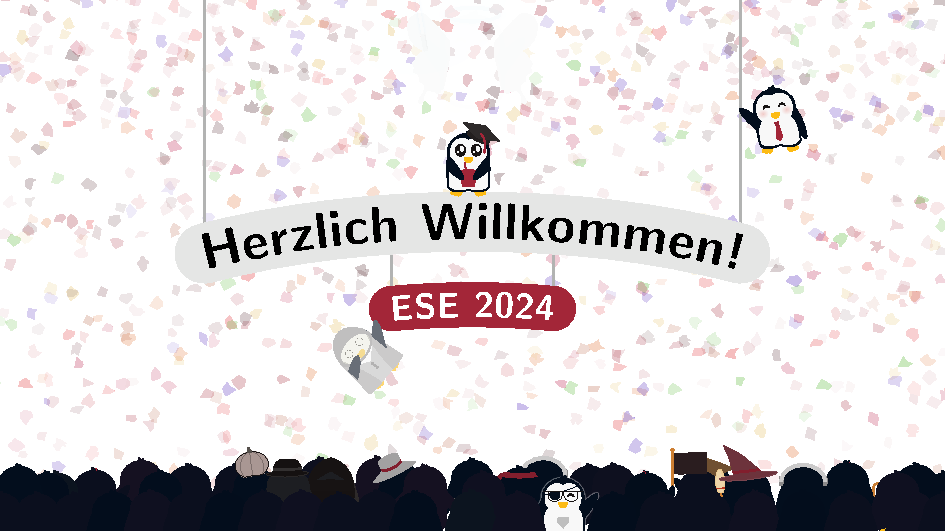
\includepdf{assets/hey}

\subsection{Bin ich hier richtig?}
\MakeNewBox{Info}{red}
\MakeNewBox{SE}{blue}
\MakeNewBox{MI}{green}
\begin{frame}{\insertsubsection}
	\begin{fancycolumns}[columns=3]
		\begin{Info}{} \begin{minipage}[c][2cm][c]{\textwidth}
            \centering
            \huge Informatik
        \end{minipage}\end{Info}
		\nextcolumn
		\begin{SE}{} \begin{minipage}[c][2cm][c]{\textwidth}
            \centering
            \huge Software Engineering
        \end{minipage}\end{SE}	
		\nextcolumn
		\begin{MI}{} \begin{minipage}[c][2cm][c]{\textwidth}
            \centering
            \huge Medien- informatik
        \end{minipage}\end{MI}	
	\end{fancycolumns}
\end{frame}

\subsection{Was erwartet euch?}
\begin{frame}{\insertsubsection}
	\begin{tabbing}
		\hspace*{2cm} \= \hspace*{6cm} \= \kill
		\Large\textbf{Montag} \\
		\\
		\textbf{Wann?} \> \textbf{Was?} \> \textbf{Wo?} \\
		09:00 Uhr \> Begrüßung \> N24 H13 \\
		10:00 Uhr \> Tutorien in Kleingruppen \> Seminarräume \\
		11:00 Uhr \> Mittagessen \> Mensa \\
		12:00 Uhr \> Tutorien in Kleingruppen \> Seminarräume \\
		13:00 Uhr \> Uniführung \> --- \\
		15:00 Uhr \> Vortrag How-To Studium \> H22 \\
		18:00 Uhr \> Analoges Netzwerken mit Grillen \> Innenhof A \\
		\\
	\end{tabbing}
\end{frame}

\subsection{Was erwartet euch?}
\begin{frame}{\insertsubsection}
	\begin{tabbing}
		\hspace*{2cm} \= \hspace*{6cm} \= \kill
		\Large\textbf{Dienstag} \\
		\\
		\textbf{Wann?} \> \textbf{Was?} \> \textbf{Wo?} \\
		09:00 Uhr \> Brunch mit Kurzvorträgen \> Seminarräume \\
		14:00 Uhr \> Rallye durch die Universität \> --- \\
		17:00 Uhr \> Abschluss \> Vor dem BeCI \\
		19:30 Uhr \> Kneipentour \> Münsterbrunnen \\
	\end{tabbing}
\end{frame}

\subsection{Wer sind wir überhaupt?}
\begin{frame}{\insertsubsection}
	\begin{fancycolumns}[columns=2]
			
\includegraphics[width=\linewidth]{assets/FIN_Logo.jpg}
		\nextcolumn
			\Large Fachschaft Informatik
			\begin{itemize}
				\item Vertretung der Studierenden
				\item Ansprechpersonen für Fragen
				\item Organisieren von Veranstaltungen 
			\end{itemize}
	\end{fancycolumns}
\end{frame}

\subsection{}
\begin{frame}{\insertsubsection}
	\begin{center}
		\Huge\textbf{Wir sind für euch da!}
	\end{center}
\end{frame}


\subsection{Wen könnt ihr ansprechen?}
\begin{frame}{\insertsubsection}
	\begin{fancycolumns}[columns=3]
		Tutorium 1
		\begin{itemize}
			\item Koko
			\item Enrique
		\end{itemize}
		Tutorium 2
		\begin{itemize}
			\item Johanna
			\item Lars
		\end{itemize}
		\nextcolumn
		Tutorium 3
		\begin{itemize}
			\item Jonas
			\item Leo
		\end{itemize}
		Tutorium 4
		\begin{itemize}
			\item Nick
			\item Laurin
		\end{itemize}
		\nextcolumn
		Tutorium 5
		\begin{itemize}
			\item Marc
			\item Johannes
		\end{itemize}
	\end{fancycolumns}
\end{frame}

\subsection{Wen könnt ihr ansprechen?}
\begin{frame}{\insertsubsection}
	\begin{fancycolumns}[columns=2]
		Tutorium 1
		\begin{itemize}
			\item Koko
			\item Enrique
		\end{itemize}
		Tutorium 2
		\begin{itemize}
			\item Johanna
			\item Laurin
		\end{itemize}
		\nextcolumn
		Tutorium 3
		\begin{itemize}
			\item Jonas
			\item Lars
		\end{itemize}
		Tutorium 4
		\begin{itemize}
			\item Marc
			\item Johannes
		\end{itemize}
	\end{fancycolumns}
\end{frame}

\end{document}